\PassOptionsToPackage{unicode=true}{hyperref} % options for packages loaded elsewhere
\PassOptionsToPackage{hyphens}{url}
\PassOptionsToPackage{dvipsnames,svgnames*,x11names*}{xcolor}
%
\documentclass[paper=a4,]{tufte-handout}
\usepackage{lmodern}
\usepackage{amssymb,amsmath}
\usepackage{cleveref}
\usepackage{ifxetex,ifluatex}
\usepackage{fixltx2e} % provides \textsubscript
\ifnum 0\ifxetex 1\fi\ifluatex 1\fi=0 % if pdftex
  \usepackage[T1]{fontenc}
  \usepackage[utf8]{inputenc}
  \usepackage{textcomp} % provides euro and other symbols
\else % if luatex or xelatex
  \usepackage{unicode-math}
  \defaultfontfeatures{Ligatures=TeX,Scale=MatchLowercase}
\fi
% use upquote if available, for straight quotes in verbatim environments
\IfFileExists{upquote.sty}{\usepackage{upquote}}{}
% use microtype if available
\IfFileExists{microtype.sty}{%
\usepackage[]{microtype}
\UseMicrotypeSet[protrusion]{basicmath} % disable protrusion for tt fonts
}{}
\IfFileExists{parskip.sty}{%
\usepackage{parskip}
}{% else
\setlength{\parindent}{0pt}
\setlength{\parskip}{6pt plus 2pt minus 1pt}
}
\usepackage{xcolor}
\usepackage{hyperref}
\hypersetup{
            pdftitle={Debugging, Tracing, and Fading: Improving the Mental Model},
            pdfauthor={Helena Rasche},
            colorlinks=true,
            linkcolor=Maroon,
            filecolor=Maroon,
            citecolor=Blue,
            urlcolor=Blue,
            breaklinks=true}
\urlstyle{same}  % don't use monospace font for urls
\usepackage{listings}
\newcommand{\passthrough}[1]{#1}
\lstset{% General setup for the package
    language=Python,
    basicstyle=\small\sffamily,
    numbers=left,
    numberstyle=\tiny,
    frame=tb,
    tabsize=4,
    columns=fixed,
    showstringspaces=false,
    showtabs=false,
    keepspaces,
    commentstyle=\color{red},
    keywordstyle=\color{blue}
}
\usepackage{graphicx,grffile}
\makeatletter
\def\maxwidth{\ifdim\Gin@nat@width>\linewidth\linewidth\else\Gin@nat@width\fi}
\def\maxheight{\ifdim\Gin@nat@height>\textheight\textheight\else\Gin@nat@height\fi}
\makeatother
% Scale images if necessary, so that they will not overflow the page
% margins by default, and it is still possible to overwrite the defaults
% using explicit options in \includegraphics[width, height, ...]{}
\setkeys{Gin}{width=\maxwidth,height=\maxheight,keepaspectratio}
\setlength{\emergencystretch}{3em}  % prevent overfull lines
\providecommand{\tightlist}{%
  \setlength{\itemsep}{0pt}\setlength{\parskip}{0pt}}
\setcounter{secnumdepth}{0}
% Redefines (sub)paragraphs to behave more like sections
\ifx\paragraph\undefined\else
\let\oldparagraph\paragraph
\renewcommand{\paragraph}[1]{\oldparagraph{#1}\mbox{}}
\fi
\ifx\subparagraph\undefined\else
\let\oldsubparagraph\subparagraph
\renewcommand{\subparagraph}[1]{\oldsubparagraph{#1}\mbox{}}
\fi

% set default figure placement to htbp
\makeatletter
\def\fps@figure{htbp}
\makeatother

\usepackage{pdfpages}

%%%%%%%%%%% Header and Footer %%%%%%%%%%%%%%%%%%
\fancyfoot[CE,CO]{\flushright 
\includegraphics[width=3cm]{../avans.jpg}}
\fancyhead[CE,CO]{\flushleft \smallcaps{\today}}

\usepackage[]{natbib}
\bibliographystyle{plainnat}

\title[]{Debugging, Tracing, and Fading: Improving the Mental Model}
\author{Helena Rasche}
\date{2022-03-21}

\begin{document}
\maketitle
\begin{abstract}
Students have a poor working model of code which leads to numerous
issues; they struggle to debug, to adjust copy-pasted code, and to
predict runtime behaviour.

Existing research provides a number of avenues for improving our coding
education and improving the student experience. Here we discuss a number
of strategies to enhance student learning, provide a deeper
understanding of code, and improve the student mental model of code
execution. This should allow students to thrive as budding coders.
\end{abstract}
\noindent\rule{5in}{0.4pt}


\hypertarget{the-problem}{%
\section{The Problem}\label{the-problem}}

Currently students finish the course with a moderate working
understanding of code, not sufficient to write their own programs or
adapt new code to their situation. This is an extremely suboptimal
outcome, after 8 weeks they should be able to write moderately complex
python programs.

Showing what happens live on the screen is received well by students, if
they can manage to watch what we type and try to type it themselves
simultaneously. We know at least that our examples give the correct
result, but students never see anything other than correct, working
code, and never have to formulate an internal model for how to write
code. They end up copying and pasting and not understanding \emph{why}.
As of now nothing is going ``well'', and there is room for improvement
in all aspects, but specifically this discussion will focus on improving
mental models of code and the potential effects on understanding code
execution.

Predicting code behaviour without running it is a key component of work
as a programmer, and a lot of the time we spend debugging relies on us
emulating the computer in our head. Without a solid mental model of code
behaviour one cannot predict how it will function in one situation, much
less other or non-standard situations. Planning for code to handle both
good and bad inputs requires some creativity and mentally planning
around expected values at various points throughout the execution.

This situation leaves students unprepared for incorrect or buggy code,
either (un)intentionally included in homework assignments, or, generated
by themselves, if they cannot identify where code will fail without
executing it.

\hypertarget{the-conclusion}{%
\section{The Conclusion}\label{the-conclusion}}

Students must develop a coherent and strong internal model of code
execution to allow them to understand code flow, fix broken code, and
debug issues.

\hypertarget{my-hypothesis}{%
\section{My Hypothesis}\label{my-hypothesis}}

Augmenting lessons with:

\begin{itemize}
\tightlist
\item
  Tracing - Stepping through the internal state
\item
  Faded examples
\item
  Debugging intentionally broken examples
\end{itemize}

Will give students enough tools to respond dynamically to failure states
with informed experience to resolve issues they encounter as
programmers.

\hypertarget{opportunities-for-improvement}{%
\section{Opportunities for
Improvement}\label{opportunities-for-improvement}}

\hypertarget{mental-model}{%
\subsection{Mental Model}\label{mental-model}}

The student's mental model of the code underlies everything they do as a
programmer, from conception to implementation to debugging to their self
efficacy:

\begin{quote}
This study shows that a well-developed and accurate mental model
directly affects course performance and also increases self efficacy,
the other key element in course performance. Given this double impact,
helping students develop good mental models should remain a goal in
introductory programming courses. \citep{Ramalingam_2004}
\end{quote}

This is a foundational skill to be able to \emph{think} through a
program, step by step, and understand how the code executes and which
variables exist when, and what their values should be. This mental
modelling allows students to predict the behaviour of a system, and when
it diverges from their prediction, recognise any potential bugs.

\hypertarget{tracing}{%
\subsection{Tracing}\label{tracing}}

\begin{figure}[ht]
\begin{lstlisting}
# Initialise our accumulator
x = 1 + 1
# Loop over our input data
for i in range(10): # 0..9
    # In-loop temporary variable
    tmp = x * 2 + i
    # Update our accumulator
    x = tmp + 1
# Output our result
print(f'The final value is {x}')
\end{lstlisting}
\caption{Example Python Code. While not representative of a real world workflow, it is useful as an illustrative example, and an example which can be given directly to beginners for them to attempt.\label{fig:code}}
\end{figure}

\begin{figure}[ht]
    \begin{tabular}{r|lll}
        Line & \texttt{i} & \texttt{x} & \texttt{tmp} \\\hline
        2    & -          & 2          & - \\
        4    & 0          & 2          & - \\
        6    & 0          & 2          & 4 \\
        8    & 0          & 5          & 4 \\
        4    & 1          & 5          & - \\
        6    & 1          & 5          & 11 \\
        8    & 1          & 12         & 11 \\
        4    & 2          & 12         & - \\
        6    & 2          & 12         & 26 \\
        8    & 2          & 27         & 26 \\
\end{tabular}
\caption{Example of a student's process tracing execution flow\label{fig:table}}
\end{figure}

While there is no bug in \cref{fig:code}, when there \emph{is} a bug
present, having students produce a table like \cref{fig:table}
significantly improves their understanding of code flow and execution
\citep{Hertz_2013}. ``Tracing'' is a valuable and easy to complete
exercise, and the results can even be checked automatically leading to
good scalability of the exercise across larger classes.

\hypertarget{faded-examples}{%
\subsection{Faded Examples}\label{faded-examples}}

Given that the students taught by Avans are primarily novice programmers
who have not read or written a programming language before, we need to
take significant care of their cognitive load. Both learning based on
problem-solving and worked examples may cause high cognitive loads for
different audiences, and exploring alternatives is important
\citep{Retnowati_2017}. Faded examples such as what is seen in
\cref{fig:fade} are exactly such an alternative, starting with a fully
worked example and removing successive components until we reach a
problem description requiring a full solution. This leads to fewer
unproductive learning events \citep{Renkl_2004}.

\begin{figure}[ht]
    \begin{minipage}[b]{\linewidth}
\begin{lstlisting}
# Write a function that multiplies two numbers
def multiply(a, b):
    c = a * b
    return c
\end{lstlisting}
    %\caption{The initial problem shows the entire solution to students}
    \end{minipage}

    \begin{minipage}[b]{\linewidth}
\begin{lstlisting}
# Write a function that adds two numbers
def add(___):
    ____
    return c
\end{lstlisting}
        %\caption{Increased fading, here we call out blanks students should fill in specifically with syntactically incorrect underscores.}
    \end{minipage}

    \begin{minipage}[b]{\linewidth}
\begin{lstlisting}
# Write a function that subtracts two numbers
\end{lstlisting}
    %\caption{Final fading, the entire problem is gone except for the description of what they need to do.}
    \end{minipage}

  \caption{Example of fading in coding exercises, these let students work on a continuum from worked out examples to self-devised solutions.\label{fig:fade}}
\end{figure}

Faded examples however, do come at a higher cost of implementation than
worked out examples \citep{Zamary_2018}. They require writing the
correct worked out example and then determining which components to
remove, which presents an additional cost during course updates that if
examples are changed they need to be double checked to ensure they are
still valid, whereas worked examples can be checked more automatically.

\hypertarget{debugging}{%
\subsection{Debugging}\label{debugging}}

Debugging is the act of identify and resolving ``bugs'' or defects
within code, a term popularly attributed to my personal hero Admiral
Grace Hopper:

\begin{quote}
While she was working on a Mark II computer at Harvard University, her
associates discovered a moth stuck in a relay and thereby impeding
operation, whereupon she remarked that they were ``debugging'' the
system \citep{enwiki:1069955193}
\end{quote}

Debugging also functions as a reinforcement method we can use once
students have an ok mental model of code execution, a necessary
pre-requisite for this activity, which can be further developed through
debugging \citep{Ramalingam_2004} alongside their self-efficacy
\citep{Michaeli_2019}. Debugging activities can take many forms but most
commonly the task is to correct incorrect code, an activity that works
best if they are primed with a number of methods of debugging
\citep{Murphy_2008} such as the ``Wolf Fence'' \citep{Gauss_1982},
commenting out code, or breakpoints.

\begin{figure}[]
\begin{lstlisting}
# Fix me!
for number in range(10):
    # use a if the number is a multiple of 3,
    # otherwise use b
    if Number % 3 == 0:
        message = message + a
    else:
        message = message + "b"
print(message)
\end{lstlisting}
\caption{A debugging exercise featuring code with numerous issues from type confusion, variable typos, and failure to initialise a variable.\label{fig:debug}}
\end{figure}

\hypertarget{pair-programming}{%
\subsection{Pair Programming}\label{pair-programming}}

\begin{figure}
\centering

\includegraphics{./pair-programming.jpg}
\caption{Pair programming has two participants join forces to develop
solutions, one leading the effort, one writing the code. (Image:
StartupStockPhotos.com / CC0)\label{fig:pair}}
\end{figure}

Complementary to the efforts of Mental Model development via
Tracing/Debugging/Fading, pair programming or ``pairing''
(\cref{fig:pair}) provides a reinforcement activity where they utilise
similar skills. As one person writes and executes code, the other person
`drives' the experience, telling them what to write
\citep{Williams,Williams_2001}. It has become a common learning
model in introductory courses due to its benefits to students
\citep{mendes2005investigating,mendes2006replicated,Hannay_2007}.
Specifically this technique has also been shown to be beneficial for
women in computer science and gives them better chances for success in
future programming endeavours \citep{werner2004pair}. Adopting this
technique already (Assignment 6) has shown initially promising results,
provided we adhere to principles outlined by \citep{Mentz_2008}.

\hypertarget{the-intervention}{%
\section{The Intervention}\label{the-intervention}}

      The intervention will consist of overhauling the formative assessments that students complete during class to include these new types of problems incorporating tracing exercises, faded examples, and debugging problems. These assessments work in unison and cannot be extracted, so they will be executed together. The example code listings provided (\cref{fig:code,fig:fade,fig:debug}) are representative of the updates to formative assessments that we will make. The choice for this specific intervention instead of pair programming\footnote{Additionally pair programming is already being trialled in one section.}

\begin{itemize}
\tightlist
\item
  This intervention is well backed by research showing improvements in
  student proficiency and grades \citep{Hertz_2013,Renkl_2002}
  leading to better learning outcomes \citep{Renkl_2004}.
\item
  These skills significantly improve self efficacy
		\citep{Ramalingam_2004,Michaeli_2019}.
\end{itemize}

The second point, lack of self-efficacy has been a significant cost for
TOAs and teachers alike in terms of interruptions for questions students
should be able to answer on their own, and by applying these
interventions hopefully students will find themselves and peers a more
reliable source of discussion and answers. Self empowerment in this
field sets the students on a good path for their future.

\hypertarget{assessment}{%
\section{Assessment}\label{assessment}}

It is difficult to conduct a sufficiently controlled experiment given
individual teacher preferences and teaching styles, so assessment will
be carried out via review of student homework solutions. The system we
use that collects student homework submission tracks student code entry
over time, and will let us review how they attempted solutions and let
us make qualitative observations.

\hypertarget{the-awaited-results}{%
\section{The Awaited Results}\label{the-awaited-results}}

\begin{figure}[ht]
\centering
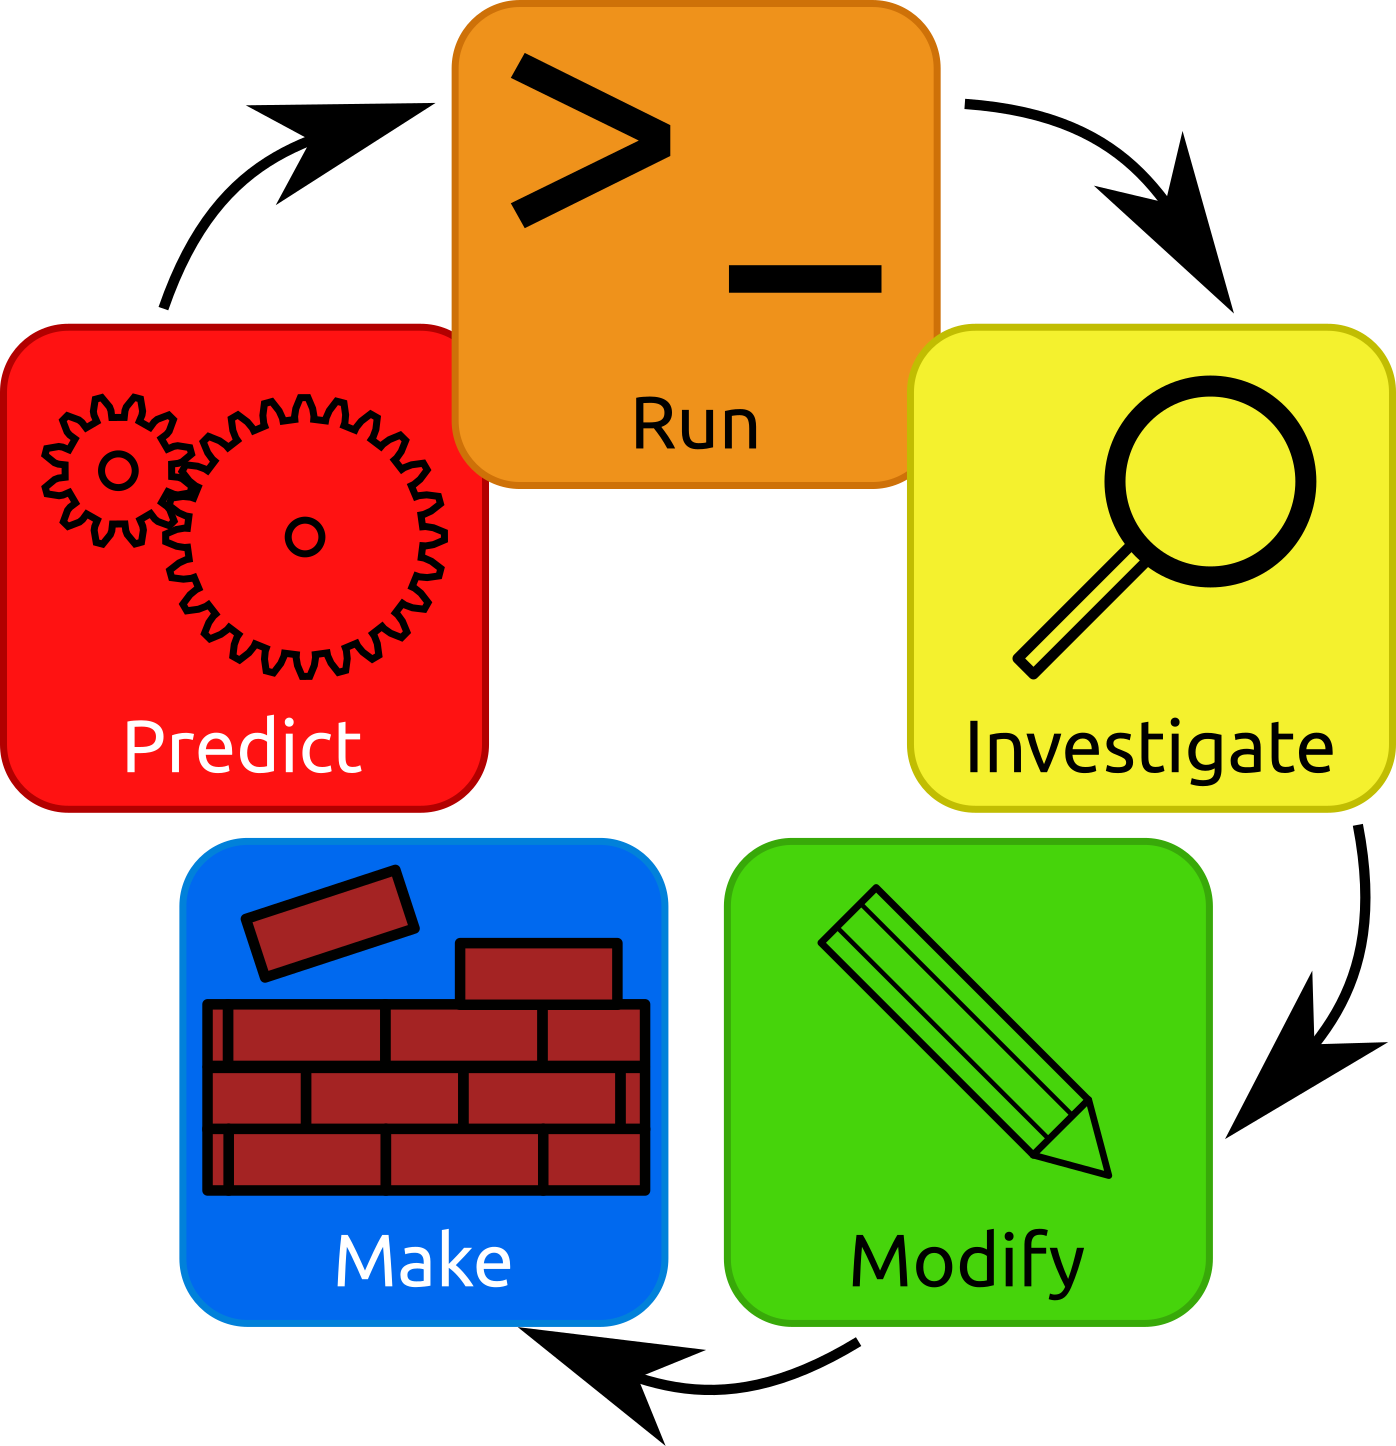
\includegraphics{./primm.png}
\caption{Diagram of the PRIMM methodology\cite{Sentance_2017}, a model incorporating all of these activities that is used in K-12 teaching, further indicating their applicability given existing educational curricula. A mental model is required to predict, tracing for investigation, debugging to modify.}
\end{figure}

Unfortunately there was not sufficient time to trial all of these
strategies and evaluate the sections. Instead, all of these are
currently being trialled in Group 32MBI02, please check back at the end
of P3 for results. It is expected that these research backed teaching
strategies will significantly improve student learning.

However, given that existing similar models, incorporating all of these
activities, is used in K-12 teaching \citep{Sentance_2017}, this
intervention is expected to produce good results. Their model, PRIMM,
starts with a good mental model which is required to predict, tracing
during investigation, and debugging to modify code, all building towards
students making things themselves.

\clearpage
\bibliography{poster.bib}

\end{document}
